%%%%%%%%%%%%%%%%%%%%%%%%%%%%%%%%%%%%%%%
% Wenneker Resume/CV
% LaTeX Template
% Version 1.1 (19/6/2016)
%
% This template has been downloaded from:
% http://www.LaTeXTemplates.com
%
% Original author:
% Frits Wenneker (http://www.howtotex.com) with extensive modifications by 
% Vel (vel@LaTeXTemplates.com)
%
% License:
% CC BY-NC-SA 3.0 (http://creativecommons.org/licenses/by-nc-sa/3.0/
%
%%%%%%%%%%%%%%%%%%%%%%%%%%%%%%%%%%%%%%

%----------------------------------------------------------------------------------------
%	PACKAGES AND OTHER DOCUMENT CONFIGURATIONS
%----------------------------------------------------------------------------------------

\documentclass[a4paper,12pt]{memoir} % Font and paper size

%%%%%%%%%%%%%%%%%%%%%%%%%%%%%%%%%%%%%%%%%
% Wenneker Resume/CV
% Structure Specification File
% Version 1.1 (19/6/2016)
%
% This file has been downloaded from:
% http://www.LaTeXTemplates.com
%
% Original author:
% Frits Wenneker (http://www.howtotex.com) with extensive modifications by 
% Vel (vel@latextemplates.com)
%
% License:
% CC BY-NC-SA 3.0 (http://creativecommons.org/licenses/by-nc-sa/3.0/)
%
%%%%%%%%%%%%%%%%%%%%%%%%%%%%%%%%%%%%%%%%%

%----------------------------------------------------------------------------------------
%	PACKAGES AND OTHER DOCUMENT CONFIGURATIONS
%----------------------------------------------------------------------------------------

\usepackage{XCharter} % Use the Bitstream Charter font
\usepackage[utf8]{inputenc} % Required for inputting international characters
\usepackage[T1]{fontenc} % Output font encoding for international characters

\usepackage[top=1cm,left=1cm,right=1cm,bottom=1cm]{geometry} % Modify margins

\usepackage{graphicx} % Required for figures

\usepackage{flowfram} % Required for the multi-column layout

\usepackage{url} % URLs

\usepackage[usenames,dvipsnames]{xcolor} % Required for custom colours

\usepackage{tikz} % Required for the horizontal rule

\usepackage{enumitem} % Required for modifying lists
\setlist{noitemsep,nolistsep} % Remove spacing within and around lists

\setlength{\columnsep}{\baselineskip} % Set the spacing between columns

% Define the left frame (sidebar)
\newflowframe{0.2\textwidth}{\textheight}{0pt}{0pt}[left]
\newlength{\LeftMainSep}
\setlength{\LeftMainSep}{0.2\textwidth}
\addtolength{\LeftMainSep}{1\columnsep}
 
% Small static frame for the vertical line
\newstaticframe{1.5pt}{\textheight}{\LeftMainSep}{0pt}
 
% Content of the static frame with the vertical line
\begin{staticcontents}{1}
\hfill
\tikz{\draw[loosely dotted,color=RoyalBlue,line width=1.5pt,yshift=0](0,0) -- (0,\textheight);}
\hfill\mbox{}
\end{staticcontents}
 
% Define the right frame (main body)
\addtolength{\LeftMainSep}{1.5pt}
\addtolength{\LeftMainSep}{1\columnsep}
\newflowframe{0.7\textwidth}{\textheight}{\LeftMainSep}{0pt}[main01]

\pagestyle{empty} % Disable all page numbering

\setlength{\parindent}{0pt} % Stop paragraph indentation

%----------------------------------------------------------------------------------------
%	NEW COMMANDS
%----------------------------------------------------------------------------------------

\newcommand{\userinformation}[1]{\renewcommand{\userinformation}{#1}} % Define a new command for the CV user's information that goes into the left column

\newcommand{\cvheading}[1]{{\Huge\bfseries\color{RoyalBlue} #1} \par\vspace{.6\baselineskip}} % New command for the CV heading
\newcommand{\cvsubheading}[1]{{\Large\bfseries #1} \bigbreak} % New command for the CV subheading

\newcommand{\Sep}{\vspace{1em}} % New command for the spacing between headings
\newcommand{\SmallSep}{\vspace{0.5em}} % New command for the spacing within headings

\newcommand{\aboutme}[2]{ % New command for the about me section
\textbf{\color{RoyalBlue} #1}~~#2\par\Sep
}
	
\newcommand{\CVSection}[1]{ % New command for the headings within sections
{\Large\textbf{#1}}\par
\SmallSep % Used for spacing
}

\newcommand{\CVItem}[2]{ % New command for the item descriptions
\textbf{\color{RoyalBlue} #1}\par
#2
\SmallSep % Used for spacing
}

\newcommand{\bluebullet}{\textcolor{RoyalBlue}{$\circ$}~~} % New command for the blue bullets
 % Include the file specifying document layout and packages

%----------------------------------------------------------------------------------------
%	NAME AND CONTACT INFORMATION 
%----------------------------------------------------------------------------------------

\userinformation{ % Set the content that goes into the sidebar of each page
\begin{flushright}
% Comment out this figure block if you don't want a photo
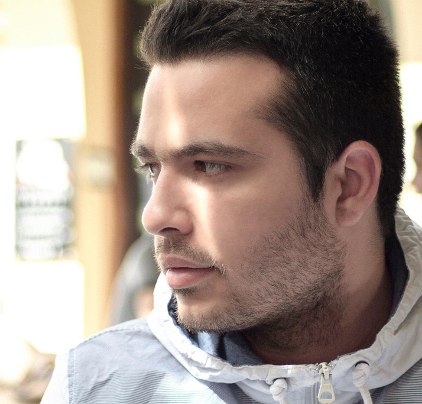
\includegraphics[width=1\columnwidth]{me.png}\\[\baselineskip] % Your photo
%\small % Smaller font size
%Paschalis Dedousis \\ % Your name
\end{flushright}
\smallskip
% image link: https://www.iconfinder.com/icons/115714/email_mail_send_icon#size=32

\includegraphics[width=0.15\columnwidth]{if_mail_115714.png}\\
\href{mailto://padedou@gmail.com}{padedou@gmail.com} \\\\ % Your email address
% image link: https://github.com/logos

\includegraphics[width=0.15\columnwidth]{GitHub-Mark-32px.png}\\
\href{https://github.com/padedou}{github.com/padedou}\\\\
%image link: https://blog.codepen.io/documentation/brand-assets/logos/

\includegraphics[width=0.15\columnwidth]{Button-Black-Large.png}\\
\href{https://codepen.io/padedou/}{codepen.io/padedou}\\\\
%image link: https://commons.wikimedia.org/wiki/File:CIS-A2K_Linkedin_Icon_(Black).svg

\includegraphics[width=0.15\columnwidth]{Linkedin.png}\\
\href{https://www.linkedin.com/in/paschalis-dedousis/}{linkedin.com/in/}\\
\href{https://www.linkedin.com/in/paschalis-dedousis/}{paschalis-dedousis}\\\\
%image link: https://commons.wikimedia.org/wiki/File:Simpleicons_Places_map-perspective-with-a-placeholder-on-it.svg

\includegraphics[width=0.15\columnwidth]{map_icon.png}\\
\href{https://www.google.com/maps/place/Serres/@41.0865858,23.5392998,15z/data=!3m1!4b1!4m5!3m4!1s0x14a9718b6729e5d5:0x9dd7c70595ce357!8m2!3d41.090923!4d23.5413198}{Currently living in:}\\
\href{https://www.google.com/maps/place/Serres/@41.0865858,23.5392998,15z/data=!3m1!4b1!4m5!3m4!1s0x14a9718b6729e5d5:0x9dd7c70595ce357!8m2!3d41.090923!4d23.5413198}{Serres, Greece}
\vfill % Whitespace under this block to push it up under the photo
%\end{flushright}
}

%----------------------------------------------------------------------------------------

\begin{document}

\userinformation % Print your information in the left column

\framebreak % End of the first column

%----------------------------------------------------------------------------------------
%	HEADING
%----------------------------------------------------------------------------------------

\cvheading{Paschalis Dedousis} % Large heading - your name

\cvsubheading{Software Developer and Engineer} % Subheading - your occupation/specialization

%----------------------------------------------------------------------------------------
%	ABOUT ME
%----------------------------------------------------------------------------------------

%----------------------------------------------------------------------------------------
%	EDUCATION
%----------------------------------------------------------------------------------------

\CVSection{Education}

%------------------------------------------------

% FCC
\CVItem{2016 - 2017, Free Code Camp}{Full Stack Web Development Certification, Software Engineering}

% TEI
\CVItem{2008 - 2016, Technological Institute of Crete} {BSc in Informatics Engineering}
\begin{itemize}
\item Thesis: \small Algorithms and processes for progressive graphics applications
\item Main courses:
		\begin{itemize}
			\item \small Plan-Driven and Agile Programming
			\item \small Computer Networks
			\item \small Internet Programming
			\item \small Multimedia Applications Programming
			\item \small Online Multimedia and Graphics
			\item \small Human Computer Interfaces
			\item \small Database Development
			\item \small Peer to Peer Networks
		\end{itemize}
\end{itemize}


%------------------------------------------------

\Sep % Extra whitespace after the end of a major section

%----------------------------------------------------------------------------------------
%	EXPERIENCE
%----------------------------------------------------------------------------------------

\CVSection{Experience}

%------------------------------------------------

\CVItem{Mar 2015 - Aug 2015, \textit{Intern Software Engineer}, iSTLab - \footnotesize Research unit of the Department of Informatics Engineering\\}{

\begin{itemize}
	\item HTML5 game editor development
	\item Multimodal interaction\\
\end{itemize}
}

%------------------------------------------------

\CVItem{Sep 2014 - present, \textit{Freelance In-Home Computer Programming Tutor\\}}{
\begin{itemize}
	\item Help university and college students succeed in their computer\\ programming courses
\end{itemize}
}

%------------------------------------------------

\Sep % Extra whitespace after the end of a major section

%----------------------------------------------------------------------------------------
%	SKILLS
%----------------------------------------------------------------------------------------

\CVSection{Software Development Skills}

%------------------------------------------------

\CVItem{Main Programming Languages, Frameworks and Technologies}
{\begin{tabular}{p{0.2\textwidth} p{0.2\textwidth} p{0.2\textwidth}}
\bluebullet Javascript &  \bluebullet X3D & \bluebullet WebGL\\
\bluebullet Three.js &  \bluebullet jQuery & \bluebullet Java\\
\bluebullet Node.js & \bluebullet 2D web games & \bluebullet Git
\end{tabular}}

%------------------------------------------------

\CVItem{Acquainted  Programming Languages, Frameworks and Technologies}
{\begin{tabular}{p{0.2\textwidth} p{0.2\textwidth} p{0.2\textwidth}}
 \bluebullet Python &  \bluebullet Django & \bluebullet Typescript\\
 \bluebullet React & \bluebullet Angular & \bluebullet CSS\\
 \bluebullet WebRTC & \bluebullet Web Audio API & \bluebullet RDBMS\\
 \bluebullet NoSQL & \bluebullet C\# & \bluebullet C/C++
\end{tabular}}

%------------------------------------------------

\Sep % Extra whitespace after the end of a major section

\end{document}
